\documentclass[11.5pt,a4paper]{article}
\usepackage[utf8]{inputenc}
\usepackage{amsmath}
\usepackage{amsfonts}
\usepackage{amssymb}
\usepackage{graphicx}
\usepackage{xcolor}
\usepackage[export]{adjustbox}
\usepackage{multicol}
\usepackage[left=2cm,right=2cm,top=2cm,bottom=2cm]{geometry}
\begin{document}

\textbf{\textcolor{gray}{\Huge Mehjebin Mujeeb}}\\ \hrule
%\textbf{\textcolor{gray}{\Huge About}}\\

\t Address: 38/ 2883 Hayath,\\ 
\t PPN Nagar ,Edappally, Kochi\\
\t Email: mehjebin.mujeeb@gmail.com\\
\t phone:+91-9495612744\\
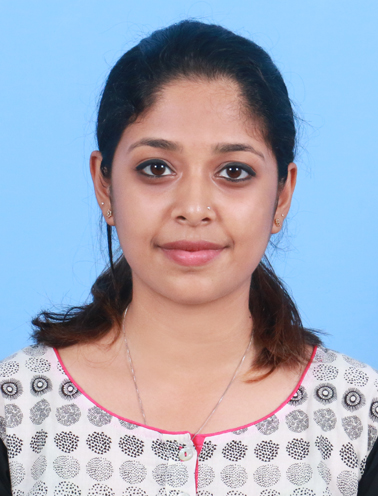
\includegraphics[scale=0.7, width=0.19\textwidth,right ]{pp}



\textbf{\textcolor{gray}{\huge Objective}}\\ \hrule
Seeking an internship position that will allow me to explore career options in the IT sector. A self-motivated, hardworking under-graduate student in computer science looking to improve technical skills.\\

\textbf{\textcolor{gray}{\huge Education}}


\begin{center}
\begin{tabular}{ |c|c|c|c|c| } 
 \hline
 \textbf{\Large Degree} &\textbf{\Large college/School}&\textbf{\Large University} & \textbf{\Large Passing year}& \textbf{\Large Pass \%} \\ \hline
BTech & FISAT,Angamaly & KTU & 2019 & 8.15(cgpa)\\ \hline
XIIth Standard & Army Public School,Pune & CBSE & 2015 & 91\% \\ \hline
Xth Standard & Army Public School,Bangalore & CBSE & 2013 & 9.4(cgpa)\\

 \hline
\end{tabular}
\end{center}

\textbf{\textcolor{gray}{\huge Projects}}\hrule
\begin{itemize}
\item[•] Multinomial Logistic Regression (Design Project)\\
       Domain – Machine learning.
\item[•] Disease Diagnosis Machine (e-Yantra Idea Competition 2018)
\end{itemize}

\textbf{\textcolor{gray}{\huge Training and Internship}}\hrule
\begin{itemize}
\item Android Application Development -\\
Learned to create a basic android app and use Android Studio.
\item Machine Learning course on Udemy
\item Web development bootcamp on Udemy (ongoing)
\end{itemize}



\end{document}